\section{Sprint 1}

\subsection*{Summary}

\begin{table}[H]
	\centering
	\begin{tabular}{ll}
		\toprule
		\multicolumn{2}{c}{\textbf{Sprint 1} \textit{(Einarbeitung \gls{dat})}}\\
		\midrule
		\textbf{Periode} & 23.02.2015\textendash 01.03.2015 12:00 Uhr\\
		\textbf{Stunden Soll} & \SI{72}{\hour}\\
		\textbf{Stunden Plan} & \SI{86.5}{\hour} \\
		\textbf{Stunden Ist} & \SI{76.5}{\hour}\\
		\bottomrule
	\end{tabular}
\end{table}

\begin{figure}[H]
	\centering
	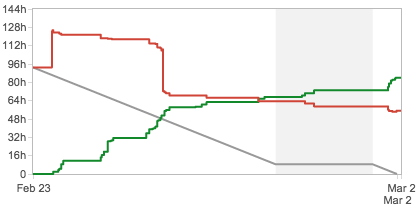
\includegraphics{fig/bd-sprint-1}
	\label{fig:pm:bd-sprint-1}
	\caption*{Burndown Chart Sprint 1}
\end{figure}

Die graue Fläche zeigt den Scope-Change aufgrund der in \cref{sec:pm:sprint1-probleme} genannten Gründe.

\subsection*{Ziele}
\begin{itemize}
	\item \Gls{dat}-Einführung abschliessen
	\item Risikoanalyse abschliessen
	\item Basis-Setup Infrastruktur abschliessen
\end{itemize}

\subsection*{Abgeschlossen}
Folgende High-level (ohne Subtasks) Jira Tasks wurden während Sprint 1 abgeschlossen.

\begin{table}[H]
\centering
\begin{tabular}{ll}
	\toprule
	\textbf{JIRA-Key} & \textbf{Summary}\\
	\midrule
	DAT-13 & Projektmeeting Woche \\
	DAT-17 & dat dokumentieren \\
	DAT-18 & Risikoanalyse \\
	DAT-19 & Infrastruktur aufsetzen \\
	DAT-24 & Übrige Aufwände Remo Sprint 1 \\
	DAT-25 & Übrige Aufwände Fabio Sprint 1 \\
	DAT-26 & Übrige Aufwände Christoph Sprint 1 \\
	DAT-30 & Sprint 0 Log\\
	\bottomrule
\end{tabular}	
\end{table}

\subsection*{Probleme}\label{sec:pm:sprint1-probleme}
Wie sich herausgestellt hat ist \gls{dat} noch nicht ansatzweise produktionsreif. Aus diesem Grund muss das ursprüngliche Ziel der Arbeit, eine Plattform basierend auf \gls{dat} zu entwickeln, angepasst werden. Die Grundidee bleibt dieselbe, nur das diese nun ohne \gls{dat} und somit mit einem komplett anderem Technologiestack umgesetzt wird. Aufgrund dieser Entscheidung wurde der Sprint vorzeitig nach einer Woche beendet und das weitere Vorgehen komplett neu geplant.